\chapter{Architektura I: trzon i blok harmoniczny}\label{rozdz:architektura}

\section{Przegląd całości}

Mamy wszystkie cegiełki: HCQT (rozdział~\ref{rozdz:hcqt}), konwolucje, LayerNorm, połączenia resztkowe (rozdział~\ref{rozdz:siec}), uwagę (rozdział~\ref{rozdz:uwaga}), straty (rozdział~\ref{rozdz:strata}). Teraz składamy z nich sieć.
W tym rozdziale opisujemy jej pierwszą połowę, która zamienia cechy HCQT na wektor opisu dla każdej pary (klatka, półton); w następnym --- drugą połowę z uwagą i głowicami.

Po tym rozdziale umiesz: (i)~narysować przepływ tensorów przez Gen~6 z kształtami, (ii)~policzyć wyjście bloku harmonicznego dla małych liczb, (iii)~uzasadnić, że blok wykrywa wzorzec nuty o dowolnej wysokości, (iv)~policzyć liczbę parametrów trzonu, bloków i zejścia.

\begin{figure*}[ht]
\centering
\begin{tikzpicture}[>=Stealth,x=1cm,y=1cm,font=\small]
  \tikzset{b/.style={blok,minimum height=11mm,minimum width=24mm,font=\small,text width=24mm,align=center},
           kszt/.style={font=\footnotesize,text=black!70}}
  \node[b] (x) at (0,0) {HCQT};
  \node[b,right=8mm of x] (stem) {trzon\\conv $3{\times}7$};
  \node[b,right=8mm of stem,fill=blue!8!white] (hb) {$3\times$ blok harmoniczny};
  \node[b,right=8mm of hb] (dw) {zejście do półtonów\\conv $1{\times}3$, krok $3$\\$+\,e_s$};
  \draw[wektor] (x)--(stem); \draw[wektor] (stem)--(hb); \draw[wektor] (hb)--(dw);
  \node[kszt,below=1mm of x] {$[B,9,T,159]$};
  \node[kszt,below=1mm of stem] {$[B,48,T,159]$};
  \node[kszt,below=1mm of hb] {$[B,48,T,159]$};
  \node[kszt,below=1mm of dw] {$[B,T,53,64]$};
  \node[b,below=17mm of x,fill=orange!10!white] (ctx) {$2\times$ warstwa kontekstu\\(uwaga w czasie\\+ uwaga między wysokościami\\+ FF)};
  \node[b,right=8mm of ctx] (ln) {LayerNorm};
  \node[b,right=8mm of ln,fill=green!8!white] (heads) {głowice:\\początek, brzmi, koniec,\\głośność, tabulatura};
  \draw[wektor] (dw.south) -- ++(0,-9mm) -| (ctx.north);
  \draw[wektor] (ctx)--(ln); \draw[wektor] (ln)--(heads);
  \node[kszt,below=1mm of ctx] {$[B,T,53,64]$};
  \node[kszt,below=1mm of ln] {$[B,T,53,64]$};
  \node[kszt,below=1mm of heads] {$[B,T,53]\ \times4,\ [B,T,6,21]$};
\end{tikzpicture}
\caption{Przepływ tensorów w Gen~6 ($B$ --- liczba nagrań w paczce, $T$ --- liczba klatek). Pierwsza połowa (rozdz.~\ref{rozdz:architektura}, niebieskie pole): cechy HCQT przechodzą przez trzon i trzy bloki harmoniczne,
a potem „schodzą” z $159$ binów do $53$ półtonów ($64$ liczby opisu na każdą parę klatka--półton). Druga połowa (rozdz.~\ref{rozdz:uwaga-wys}): dwie warstwy kontekstu (pomarańczowe pole), normalizacja i pięć głowic (zielone pole). Łącznie $249\,219$ parametrów.}
\label{rys:architektura}
\end{figure*}

\section{Trzon}

Trzon to pojedyncza konwolucja $3\times7$ (rozdział~\ref{rozdz:siec}) z $9$ kanałów HCQT do $H=48$ kanałów, po której stosujemy GELU:
$h^{(0)}=\GELU\big(\Conv_{3\times7}(X)\big)\in\R^{48\times T\times159}$. Jądro ma $3$ klatki w czasie i $7$ binów ($\approx2$ półtony) po wysokości: łączy sąsiednie klatki i sąsiednie biny, ucząc się prostych wzorców (wzrost energii, pik, cienkie prążki).
Parametrów: $9\cdot48\cdot21+48=9120$ (przykład z rozdziału~\ref{rozdz:siec}).

\section{Blok harmoniczny}

To najważniejsza nowość Gen~6. Z rozdziału~\ref{rozdz:alikwoty} wiemy, że alikwoty nuty o numerze binu $p$ leżą w binach $p+k_h$ z $k_h=\round(36\log_2h)$. Przesunięcia dla $h=0{,}5;1;2;3;4;5;6$ to
$K=(-36,0,36,57,72,84,93)$ (wniosek~\ref{wn:biny}). Blok pozwala jednej warstwie zobaczyć wszystkie te miejsca naraz.

\haslo{przesunięcie po wysokości}
\begin{definicja}[Operator przesunięcia]\label{def:shift}
Dla tensora $h\in\R^{H\times T\times P}$ i całkowitego $k$ definiujemy $\shift_k(h)[c,t,p]=h[c,t,p+k]$, a wartości spoza zakresu $0\le p+k<P$ zastępujemy zerami.
\end{definicja}

\begin{przyklad}\label{prz:shift}
Dla jednego kanału i jednej klatki: $x=(1,2,3,4,5,6,7,8)$, $k=2$: $\shift_2(x)=(3,4,5,6,7,8,0,0)$; $k=-2$: $\shift_{-2}(x)=(0,0,1,2,3,4,5,6)$. Wartość na pozycji $p$ to wartość z pozycji $p+k$; na brzegach wchodzi zero.
\end{przyklad}

Blok harmoniczny o wejściu $x\in\R^{H\times T\times P}$ liczy (z $H=48$, $7$ przesunięciami, $d$ --- dylatacja czasowa):
\begin{align}
\tilde h &= \LN_\mathrm{kan}(x), \qquad u=W_h\,\big[\shift_{k_1}(\tilde h)\,\Vert\cdots\Vert\,\shift_{k_7}(\tilde h)\big],\\
v &= \GELU\!\Big(\DW_{1\times5}\big(\GELU(u)\big)\Big), \qquad
y=x+\Drop\Big(\GELU\big(\Conv^{(d)}_{3\times1}(v)\big)\Big).
\end{align}
Znaczenie symboli: $\LN_\mathrm{kan}$ --- LayerNorm po $H$ kanałach w każdym punkcie $(t,p)$ osobno; $\Vert$ --- sklejenie wzdłuż osi kanałów (siedem kopii po $48$ daje $336$ kanałów); $W_h$ --- konwolucja $1\times1$ ($336\to48$), czyli ta sama warstwa liniowa w każdym punkcie;
$\DW_{1\times5}$ --- konwolucja głębokościowa po $5$ sąsiednich binach (na rozstrojenie i nieharmoniczność, por.\ rozdział~\ref{rozdz:alikwoty}); $\Conv^{(d)}_{3\times1}$ --- konwolucja w czasie z dylatacją $d\in\{1,2,4\}$ w kolejnych blokach.

\begin{naliczbach}
Mały model bloku: jeden kanał, jedna klatka, $x=(1,\dots,8)$, dwa przesunięcia $k\in\{0,2\}$, $W_h=(0{,}5;\ 1)$ (czyli $u[p]=0{,}5\,x[p]+1\cdot x[p+2]$), $b=0$.
Z przykładu~\ref{prz:shift}: $\shift_0(x)=x$, $\shift_2(x)=(3,4,5,6,7,8,0,0)$, więc
$u=(0{,}5\cdot1+3,\ 0{,}5\cdot2+4,\dots)=(3{,}5;\ 5;\ 6{,}5;\ 8;\ 9{,}5;\ 11;\ 3{,}5;\ 4)$.
Pozycja $p$ „widzi” teraz jednocześnie siebie i miejsce o $2$ dalej; w prawdziwym bloku to miejsca $p-36,p,p+36,p+57,\dots,p+93$, a wagi $W_h$ są uczone.
\end{naliczbach}

\begin{intuicja}
W pozycji $p$ (kandydat na podstawową) blok dostaje jednocześnie energię z siedmiu miejsc: subharmonicznej, podstawy i alikwotów od drugiego do szóstego. $W_h$ uczy się „wzorca nuty”: duża wartość w kilku z tych miejsc naraz świadczy o nucie w $p$.
Ponieważ oś jest logarytmiczna, wzorzec jest ten sam dla każdej wysokości (tw.~\ref{tw:wzorzec}), więc jedna wspólna $W_h$ działa wszędzie. To „zszycie” alikwotów w jedną kolumnę robi z błędu oktawowego problem uczenia, a nie kombinatoryki.
\end{intuicja}

\begin{twierdzenie}[Blok harmoniczny jest równoważny przesunięciom wysokości]\label{tw:rownowaznosc-wysokosci}
Niech $x'[c,t,p]=x[c,t,p-s]$ (wejście przesunięte w górę o $s$ binów). Wtedy wyjście bloku harmonicznego spełnia $y'[c,t,p]=y[c,t,p-s]$ dla wszystkich $p$ oddalonych od brzegu zakresu na tyle, że żaden z użytych indeksów $p-s+k_j$, $p-s\pm2$ nie wychodzi poza $\{0,\dots,P-1\}$.
\end{twierdzenie}
\begin{pomyslDowodu}
Każda operacja bloku jest albo punktowa (działa w każdym punkcie niezależnie), albo splotem lub przesunięciem po $p$, albo splotem w czasie; wszystkie przemieniają się z przesunięciem po $p$. Złożenie takich operacji też.
\end{pomyslDowodu}
\begin{proof}
Oznaczmy przesunięcie $(S_sx)[p]=x[p-s]$. Sprawdzamy każdy krok (z dala od brzegu, gdzie dopełnienie zerami nie gra roli):
\begin{align*}
\LN_\mathrm{kan}(S_sx) &= S_s\LN_\mathrm{kan}(x) && \pow{(osobno w każdym $(t,p)$)}\\
\shift_k(S_sx)[p] &= x[p+k-s]=(S_s\shift_kx)[p] && \pow{(def.~\ref{def:shift})}\\
W_h,\ \GELU,\ \Drop &\ \text{działają punktowo} && \pow{(przemienne z $S_s$)}\\
\DW_{1\times5}(S_sx) &= S_s\DW_{1\times5}(x) && \pow{(tw.~\ref{tw:rownowaznosc})}\\
\Conv_{3\times1}(S_sx) &= S_s\Conv_{3\times1}(x) && \pow{(czas, nie $p$)}
\end{align*}
Składanie operacji przemiennych z $S_s$ daje operację przemienną z $S_s$, a dodanie $x$ (połączenie resztkowe) też zachowuje tę własność. Stąd $y'=S_sy$. To kończy dowód.
\end{proof}

W zwykłym języku: jeśli ta sama nuta zagrana jest o $s$ binów wyżej, blok widzi dokładnie ten sam wzorzec, przesunięty o $s$. Dlatego sieć nie musi uczyć się osobnych detektorów dla każdej z $53$ nut. Cena: nic nie wie o \emph{bezwzględnej} wysokości (np.\ że niskie nuty gitary brzmią inaczej niż wysokie)
--- tę wiedzę wprowadzamy dopiero przy zejściu do półtonów, dodając wyuczone osadzenie wysokości.

\begin{figure*}[ht]
\centering
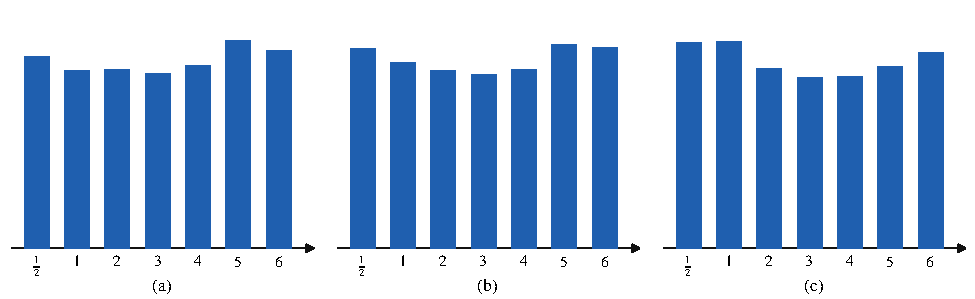
\includegraphics[width=\linewidth]{figures/harm-wagi.pdf}
\caption{Średnie wartości bezwzględne wag $W_h$ w grupach wejść odpowiadających alikwotom $h=\tfrac12,1,2,3,4,5,6$ (pod słupkami) dla trzech bloków (a), (b), (c) prawdziwego, wytrenowanego modelu Gen~6 (skala pionowa wspólna, od zera).
Wszystkie siedem miejsc ma wagi podobnej wielkości ($0{,}088$--$0{,}107$): żadne nie zostało „wyłączone”. Wielkość wag nie dowodzi jednak ważności (brak badania ablacyjnego, zob.\ rozdział~\ref{rozdz:wyniki}).}
\label{rys:harm-wagi}
\end{figure*}

\section{Zejście do półtonów}

Po trzech blokach tensor ma $159$ binów na wysokość; chcemy po jednym wektorze na półton. Konwolucja $1\times3$ z krokiem $3$ w osi wysokości (każde wyjście widzi biny $3s,3s+1,3s+2$) zmienia liczbę kanałów z $48$ na $D=64$.
Dodajemy wyuczony wektor $e_s\in\R^{64}$ dla każdego półtonu:
\begin{equation}
  h^{(1)}_{t,s}=\Conv_{1\times3,\ \text{krok }3}(y)_{t,s}+e_s\in\R^{64},\qquad s=0,\dots,52.
\end{equation}
Parametrów: konwolucja $48\cdot64\cdot3+64=9280$ i osadzenie $53\cdot64=3392$.

\begin{przyklad}\label{prz:zejscie}
Dla E2 ($s=4$) wyjście widzi biny $12,13,14$ (środek $13$, rozdział~\ref{rozdz:hcqt}). Ponieważ bloki harmoniczne wcześniej przepuściły informację z binów $p+36,\dots,p+93$ do $p$, wektor $h^{(1)}_{t,4}$ niesie wiedzę o alikwotach E2 aż do szóstego.
\end{przyklad}

\begin{naliczbach}
Parametry pierwszej połowy: trzon $9120$; blok harmoniczny: LN $2\cdot48=96$, $W_h$ $336\cdot48+48=16\,176$, $\DW$ $48\cdot5+48=288$, $\Conv_{3\times1}$ $48\cdot48\cdot3+48=6960$, razem $23\,520$ na blok i $70\,560$ w trzech;
zejście $9280$; osadzenie $3392$. Suma $9120+70\,560+9280+3392=92\,352$. Resztę ($249\,219-92\,352=156\,867$) stanowią warstwy kontekstu, LN i głowice (rozdział~\ref{rozdz:uwaga-wys}). Liczby te są sprawdzone programem względem prawdziwego modelu.
\end{naliczbach}

\begin{pulapka}
Operator $\shift_k$ wprowadza zera poza zakresem, więc dla nut o skrajnych wysokościach część alikwotów jest niewidoczna: wynik bloku dla najwyższych półtonów opiera się na mniejszej liczbie miejsc.
Tw.~\ref{tw:rownowaznosc-wysokosci} obowiązuje tylko \emph{z dala od brzegów}; sieć uczy się radzić sobie z brzegiem przez osadzenie wysokości $e_s$.
\end{pulapka}

\section*{Podsumowanie}
\begin{itemize}
\item Gen~6 to złożenie: trzon $\to$ $3\times$ blok harmoniczny $\to$ zejście do półtonów $\to$ $2\times$ warstwa kontekstu $\to$ LN $\to$ głowice (rys.~\ref{rys:architektura}).
\item Blok harmoniczny skleja $7$ przesuniętych kopii cech ($-36,0,36,57,72,84,93$ binów) i łączy je warstwą $1\times1$; jest równoważny przesunięciom po wysokości (tw.~\ref{tw:rownowaznosc-wysokosci}).
\item Trzon ma $9120$ parametrów, blok $23\,520$ (razem $70\,560$), zejście $9280$, osadzenie wysokości $3392$.
\item Kształt po zejściu: $[B,T,53,64]$ --- wektor $64$ liczb na każdą parę klatka--półton.
\end{itemize}

\begin{sprawdz}
\begin{enumerate}
\item Policz $\shift_{3}(x)$ i $\shift_{-1}(x)$ dla $x=(2,4,6,8,10)$.
\item Dla $x=(1,2,3,4,5,6)$, przesunięć $k\in\{0,3\}$ i wag $W_h=(1;\,-1)$ policz $u[p]=x[p]-x[p+3]$.
\item Ile parametrów miałby blok harmoniczny, gdyby zamiast $7$ przesunięć użyć $5$ (reszta bez zmian)?
\item Dlaczego w tw.~\ref{tw:rownowaznosc-wysokosci} nie można pominąć założenia o oddaleniu od brzegu? Podaj przykład.
\end{enumerate}
\end{sprawdz}

\subsection*{Rozwiązania}
\begin{enumerate}
\item $\shift_3(x)=(8,10,0,0,0)$; $\shift_{-1}(x)=(0,2,4,6,8)$.
\item $\shift_3(x)=(4,5,6,0,0,0)$, więc $u=(1-4,\,2-5,\,3-6,\,4-0,\,5-0,\,6-0)=(-3,-3,-3,4,5,6)$.
\item $W_h$ zmieni się na $5\cdot48\to48$: $240\cdot48+48=11\,568$ (zamiast $16\,176$); pozostałe: LN $96$, $\DW$ $288$, $\Conv_{3\times1}$ $6960$; razem $18\,912$.
\item Dla $p$ blisko brzegu np.\ $p+k_j\ge P$ i $\shift$ wstawia zero zamiast wartości z poza zakresu. Wejście przesunięte o $s$ ma w tym miejscu \emph{prawdziwą} wartość, a nieprzesunięte zero (lub odwrotnie), więc wyjścia różnią się.
\end{enumerate}
